\documentclass[11pt]{article}
\usepackage[colorlinks,urlcolor=blue,linkcolor=blue,citecolor=blue]{hyperref}
% \usepackage[footnotesize]{subfigure}
\usepackage{graphicx}
\usepackage{verbatim}
\usepackage{verbments}
\setlength{\oddsidemargin}{-0.01in}
\setlength{\topmargin}{-0.4in}
\setlength{\textheight}{9.0in}
\setlength{\textwidth}{6.5 in}

\date{December 2013}

%  \topmargin 0.in  \headheight 0pt  \headsep 0pt  \raggedbottom
%  \oddsidemargin 0.1in
%  \textheight 9.25in  \textwidth 6.00in
%  \parskip 5pt plus 1pt minus 1pt
%  \def \baselinestretch {1.25}   % one-and-a-half spaced
%  \setlength {\unitlength} {0.75in}
%
%
\newenvironment{routine}[2]
{\vspace{.0in}{\noindent\bf\hspace{-5pt}  #1}{\\ \noindent #2}
\begin{list}{}{
\renewcommand{\makelabel}[1]{{\tt  ##1 } \hfil}
\itemsep 0pt plus 1pt minus 1pt
\leftmargin  1.5in
\rightmargin 0.0in
\labelwidth  1.1in
\itemindent  0.0in
\listparindent  0.0in
\labelsep    0.05in}
}{\end{list}}
%


%


\begin{document}

\title{OP2 C++ User's Manual}
\author{Mike Giles, Gihan R. Mudalige, Istv{\'a}n Reguly}
\maketitle

\newpage




\tableofcontents

\newpage

\newpage
\section{Introduction}

OP2 is a high-level framework with associated libraries and
preprocessors to generate parallel executables for applications
on unstructured grids.  This document describes the C++ API,
but FORTRAN 90 is also supported with a very similar API.

The key concept behind OP2 is that unstructured grids can be
described by a number of sets.  Depending on the application,
these sets might be of nodes, edges, faces, cells of a variety
of types, far-field boundary nodes, wall boundary faces, etc.
Associated with these are data (e.g.~coordinate data at nodes)
and mappings to other sets (e.g.~edge mapping to the two nodes
at each end of the edge).  All of the numerically-intensive
operations can then be described as a loop over all members of
a set, carrying out some operations on data associated directly
with the set or with another set through a mapping.

OP2 makes the important restriction that the order in which the
function is applied to the members of the set must not affect the
final result to within the limits of finite precision floating-point arithmetic.
This allows the parallel implementation to choose
its own ordering to achieve maximum parallel efficiency.
Two other restrictions are that the sets and maps are static
(i.e.~they do not change) and the operands in the set operations
are not referenced through a double level of mapping indirection
(i.e.~through a mapping to another set which in turn uses another
mapping to data in a third set).

OP2 currently enables users to write a single program which can be
built into three different executables for different single-node
platforms:
\begin{itemize}
\item
single-threaded on a CPU
\item
parallelised using CUDA for NVIDIA GPUs
\item
multi-threaded using OpenMP for multicore CPU systems
\end{itemize}

\noindent A current development branch, also supports AVX vectorisation for x86 CPUs, and OpenCL for both CPUs and
GPUS. In addition to this, there is support for distributed-memory MPI parallelisation in combination with any of the
above.  The user can either use OP2's parallel file I/O capabilities for HDF5 files with a specified structure, or
perform their own parallel file I/O using custom MPI code.

\newpage
\section{Overview}

A computational project can be viewed as involving three steps:
\begin{itemize}
\item
writing the program
\item
debugging the program, often using a small testcase
\item
running the program on increasingly large applications
\end{itemize}

\noindent With OP2 we want to simplify the first two tasks, while
providing as much performance as possible for the third.

To achieve the high performance for large applications, a
preprocessor is needed to generate the CUDA code for GPUs
or OpenMP code for multicore x86 systems.  However, to keep
the initial development simple, a development single-threaded executable
can be created without any special tools; the user's main code is simply
linked to a set of library routines, most of which do little
more than error-checking to assist the debugging process by
checking the correctness of the user's program.  Note that this
single-threaded version will not execute efficiently.  The
preprocessor is needed to generate efficient single-threaded and OpenMP code for
CPU systems.\\

\noindent Figure \ref{fig:seq} shows the build process for a single
thread CPU executable.  The user's main program (in this case
{\tt jac.cpp}) uses the OP2 header file {\tt op\_seq.h} and is
linked to the appropriate OP2 libraries using {\tt g++},
perhaps controlled by a Makefile.\\

\noindent Figure \ref{fig:cuda} shows the build process for the corresponding
CUDA executable.  The preprocessor parses the user's main program
and produces a modified main program and a CUDA file which
includes a separate file for each of the kernel functions.  These
are then compiled and linked to the OP libraries
using {\tt g++} and the NVIDIA CUDA compiler {\tt nvcc}, again
perhaps controlled by a Makefile.\\

\noindent Figure \ref{fig:op} shows the OpenMP build process which is very
similar to the CUDA process except that it uses {\tt *.cpp} files
produced by the preprocessor instead of {\tt *.cu} files.\\

In looking at the API specification, users may think it is
a little verbose in places. e.g.~users have to re-supply
information about the datatype of the datasets being used
in a parallel loop.  This is a deliberate choice to simplify
the task of the preprocessor, and therefore hopefully reduce
the chance for errors.  It is also motivated by the thought that
{\bf ``programming is easy; it's debugging which is difficult''}.
i.e.~writing code isn't time-consuming, it's correcting it
which takes the time.  Therefore, it's not unreasonable to ask
the programmer to supply redundant information, but be assured
that the preprocessor or library will check that all redundant
information is self-consistent.  If you declare a dataset as being
of type {\tt OP\_DOUBLE} and later say that it is of type
{\tt OP\_FLOAT} this will be flagged up as an error at run-time.

\newpage

% \begin{comment}
\begin{figure}
\begin{center}
{\setlength{\unitlength}{1in}
\begin{picture}(4.5,2)

\put(-0.2,1.6){\framebox(0.8,0.3){\tt op\_seq.h}}
\put(1,1.5){\framebox(1,0.5){\tt jac.cpp}}

\put(0.65,1.75){\line(1,0){0.1}}
\put(0.85,1.75){\vector(1,0){0.1}}

\put(2.5,1.5){\framebox(1,0.5){\tt libraries}}

\put(1.5,1.5){\vector(0,-1){0.625}}

\put(3,1.5){\vector(0,-1){0.625}}

\put(2.25,0.5){\oval(2.5,0.75)}
\put(2.25,0.5){\makebox(0,0){make / g++}}

\end{picture}}
\end{center}

\caption{Build process for the development single threaded CPU version}
\label{fig:seq}
\end{figure}
% \end{comment}


% \begin{figure}[ht]\centering\vspace{0pt}
% \subfigure[Single-Node build]{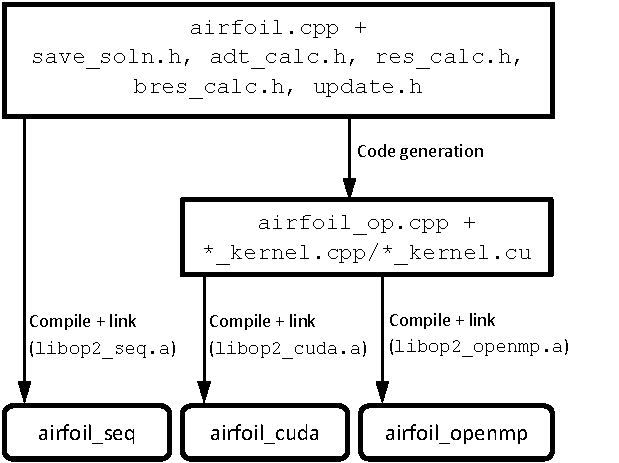
\includegraphics[width=9cm]{airfoil_plain}\vspace{-0pt}}
% \subfigure[MPI Build]{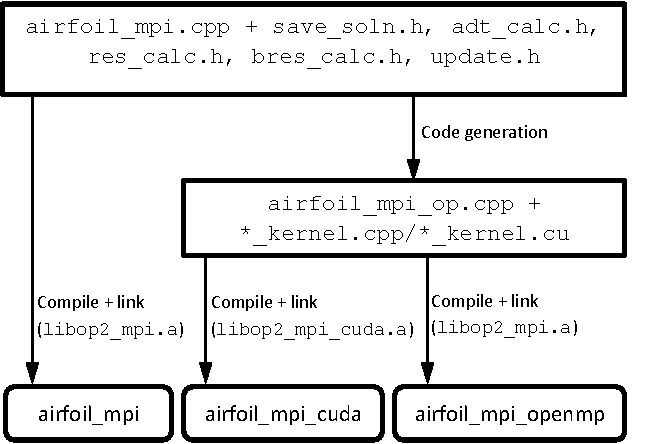
\includegraphics[width=9cm]{airfoil_plain_mpi}\vspace{-0pt}}
% \caption{Code generation and build for Airfoil (with user I/O)}\label{fig/build-paths}\vspace{-5pt}
% \end{figure}



\begin{figure}
\begin{center}
{\setlength{\unitlength}{1in}
\begin{picture}(7,5)

\put(1.5,4){\framebox(1,0.5){\tt jac.cpp}}

\put(2.0,4.0){\vector(0,-1){0.625}}

\put(2.1,3.0){\oval(4.2,0.75)}
\put(2.1,3.0){\makebox(0,0){preprocessor / code generator}}

\put(0.5,2.625){\vector(0,-1){0.625}}
\put(2.0,2.625){\vector(0,-1){0.625}}
\put(3.5,2.625){\vector(0,-1){0.625}}

\put(0.0,1.5){\framebox(1,0.5){\tt jac\_op.cpp}}
\put(1.3,1.5){\framebox(1.2,0.5){\tt jac\_kernels.cu}}
\put(2.8,1.5){\framebox(1.4,0.5){}}
\put(3.5,1.85){\makebox(0,0){\tt res\_kernel.cu}}
\put(3.5,1.65){\makebox(0,0){\tt update\_kernel.cu}}
\put(4.5,1.5){\framebox(1,0.5){\tt libraries}}

\put(0.5,1.5){\vector(0,-1){0.625}}
\put(2.0,1.5){\vector(0,-1){0.625}}
\put(5.0,1.5){\vector(0,-1){0.625}}

\put(2.62,1.75){\vector(-1,0){0.1}}
\put(2.78,1.75){\line(-1,0){0.1}}


\put(2.75,0.5){\oval(5.5,0.75)}
\put(2.75,0.5){\makebox(0,0){make / nvcc / g++}}

\end{picture}}
\end{center}

\caption{CUDA code build process}
\label{fig:cuda}
\end{figure}



\begin{figure}
\begin{center}
{\setlength{\unitlength}{1in}
\begin{picture}(7,5)

\put(1.5,4){\framebox(1,0.5){\tt jac.cpp}}

\put(2.0,4.0){\vector(0,-1){0.625}}

\put(2.1,3.0){\oval(4.2,0.75)}
\put(2.1,3.0){\makebox(0,0){preprocessor / code generator}}

\put(0.5,2.625){\vector(0,-1){0.625}}
\put(2.0,2.625){\vector(0,-1){0.625}}
\put(3.5,2.625){\vector(0,-1){0.625}}

\put(0.0,1.5){\framebox(1,0.5){\tt jac\_op.cpp}}
\put(1.3,1.5){\framebox(1.2,0.5){\tt jac\_kernels.cpp}}
\put(2.8,1.5){\framebox(1.4,0.5){}}
\put(3.5,1.85){\makebox(0,0){\tt res\_kernel.cpp}}
\put(3.5,1.65){\makebox(0,0){\tt update\_kernel.cpp}}
\put(4.5,1.5){\framebox(1,0.5){\tt libraries}}

\put(0.5,1.5){\vector(0,-1){0.625}}
\put(2.0,1.5){\vector(0,-1){0.625}}
\put(5.0,1.5){\vector(0,-1){0.625}}

\put(2.62,1.75){\vector(-1,0){0.1}}
\put(2.78,1.75){\line(-1,0){0.1}}


\put(2.75,0.5){\oval(5.5,0.75)}
\put(2.75,0.5){\makebox(0,0){make / icc}}

\end{picture}}
\end{center}

\caption{OpenMP code build process}
\label{fig:op}
\end{figure}


\clearpage

\newpage
\section{OP2 C++ API}

\subsection{Initialisation and termination routines}
\subsubsection*{}\addcontentsline{toc}{subsubsection}{op\_init}
\begin{routine} {void op\_init(int argc, char **argv, int diags\_level)}
{This routine must be called before all other OP routines. Under MPI back-ends, this routine also calls
\texttt{MPI\_Init()} unless its already called previously}
\item[argc, argv]   the usual command line arguments
\item[diags\_level] an integer which defines the level of debugging
                    diagnostics and reporting to be performed;
                    \\0 -- none;
                    \\1 -- error-checking;
                    \\2 -- info on plan construction;
                    \\3 -- report execution of parallel loops;
                    \\4 -- report use of old plans;
                    \\7 -- report positive checks in op\_plan\_check;
\end{routine}


\subsubsection*{}\addcontentsline{toc}{subsubsection}{op\_exit}
\begin{routine} {void op\_exit()}
{This routine must be called last to cleanly terminate the OP computation. Under MPI back-ends, this routine also calls
\texttt{MPI\_Finalize()} unless its has been called previously. A runtime error will occur if \texttt{MPI\_Finalize()}
is called after \texttt{op\_exit()}}
\item \vspace{-0.4in}
\end{routine}

\subsubsection*{}\addcontentsline{toc}{subsubsection}{op\_decl\_set}
\begin{routine} {op\_set op\_decl\_set(int size, char *name)}
{This routine defines a set, and returns a set ID.}

\item[size]          number of elements in the set
\item[name]          a name used for output diagnostics
\end{routine}

\subsubsection*{}\addcontentsline{toc}{subsubsection}{op\_decl\_map}
\begin{routine} {op\_map op\_decl\_map(op\_set from, op\_set to, int dim, int *imap, char *name)}
{This routine defines a mapping from one set to another, and returns a map ID.}

\item[from]          set pointed from
\item[to]            set pointed to
\item[dim]           number of mappings per element
\item[imap]          input mapping table
\item[name]          a name used for output diagnostics
\end{routine}

\newpage

\subsubsection*{}\addcontentsline{toc}{subsubsection}{op\_decl\_const}
\begin{routine} {void op\_decl\_const(int dim, char *type, T *dat, char *name)}
{This routine declares constant data with global scope to be used in user's kernel
functions. Note: in sequential version, it is the user's responsibility to define the
appropriate variable with global scope.}

\item[dim]           dimension of data (i.e.~array size)

                     for maximum efficiency, this should be a literal constant
                     (i.e. a number not a variable)

\item[type]          datatype, either intrinsic (``float'', ``double'', ``int'', ``uint'',
                     ``ll'', ``ull'' or ``bool'') or user-defined
\item[dat]          input data of type {\tt T}  (checked for consistency with {\tt type} at run-time)
\item[name]          global name to be used in user's kernel functions;\\
                     a scalar variable if {\tt dim=1}, otherwise an array of size {\tt dim}
\end{routine}

\subsubsection*{}\addcontentsline{toc}{subsubsection}{op\_decl\_dat}
\begin{routine} {op\_dat op\_decl\_dat(op\_set set, int dim, char *type, T *data, char *name)}
{This routine defines a dataset, and returns a dataset ID.}

\item[set]           set
\item[dim]           dimension of dataset (number of items per set element)

                     at present this must be a literal constant (i.e. a number not a variable);
                     this restriction will be removed in the future but a literal constant will
                     remain more efficient
\item[type]          datatype, either intrinsic or user-defined -- expert users can add a qualifier to control data
layout and management within OP2 (see section \ref{sec:expert})
\item[data]          input data of type {\tt T}  (checked for consistency with {\tt type} at run-time) -- for each
element in {\tt set}, the {\tt dim} data items muct be contiguous, but OP2 may use a different data layout internally
for better performance on certain hardware platforms (see section \ref{sec:expert})
\item[name]          a name used for output diagnostics
\end{routine}


\newpage

\subsubsection*{}\addcontentsline{toc}{subsubsection}{op\_decl\_dat\_tmp}
\begin{routine} {op\_dat op\_decl\_dat\_tmp(op\_set set, int dim, char *type, char *name)}
{This routine defines a temporary dataset, initialises it to zero, and returns a dataset ID.}

\item[set]           set
\item[dim]           dimension of dataset (number of items per set element)

                     at present this must be a literal constant (i.e. a number not a variable);
                     this restriction will be removed in the future but a literal constant will
                     remain more efficient
\item[type]          datatype, either intrinsic or user-defined -- expert users can add a qualifier to control data layout and management within OP2 (see section \ref{sec:expert})
\item[name]          a name used for output diagnostics
\end{routine}

\subsubsection*{}\addcontentsline{toc}{subsubsection}{op\_free\_dat\_tmp}
\begin{routine} {void op\_free\_dat\_tmp(op\_dat dat)}
{This routine terminates a temporary dataset.}
\item[dat]           OP dataset ID
\end{routine}

\subsubsection*{}\addcontentsline{toc}{subsubsection}{op\_diagnostic\_output}
\begin{routine} {void op\_diagnostic\_output()}
{This routine prints out various useful bits of diagnostic info about sets, mappings and datasets}
\item \vspace{-0.3in}
\end{routine}

%\vspace{0.5in}
%
%In the future there will be a new function {\tt \bf op\_partition} which
%will re-number all of the elements in each set to maximise the data reuse
%within each mini-partition.  This may be based on recursive geometric bisection
%if the user is able to supply coordinate data for one of the sets.

\newpage

\subsection{Parallel loop syntax}

A parallel loop with N arguments has the following syntax:

\subsubsection*{}\addcontentsline{toc}{subsubsection}{op\_par\_loop}
\begin{routine} {void op\_par\_loop(void (*kernel)(...), char *name, op\_set set,\\
\hspace*{1.35in}    op\_arg arg1, op\_arg arg2, \ldots , op\_arg argN)}{}

\item[kernel]     user's kernel function with N arguments\\
                  (this is only used for the single-threaded CPU build)
\item[name]       name of kernel function, used for output diagnostics
\item[set]        OP set ID
\item[args]       arguments
\end{routine}


\vspace{0.4in}
\noindent
The {\bf op\_arg} arguments in {\bf op\_par\_loop} are provided by one of the
following routines, one for global constants and reductions, and the other
for OP2 datasets.  In the future there will be a third one for sparse matrices
to support the needs of finite element calculations.

\vspace{0.2in}

\subsubsection*{}\addcontentsline{toc}{subsubsection}{op\_arg\_gbl}
\begin{routine} {op\_arg op\_arg\_gbl(T *data, int dim, char *typ, op\_access acc)}{}
\item[data]       data array
\item[dim]        array dimension
\item[typ]        datatype (redundant info, checked at run-time for consistency)
\item[acc]        access type:\\
                  {\tt OP\_READ}: read-only\\
                  {\tt OP\_INC}: global reduction to compute a sum\\
                  {\tt OP\_MAX}: global reduction to compute a maximum \\
                  {\tt OP\_MIN}: global reduction to compute a minimum
\end{routine}

\newpage

\subsubsection*{}\addcontentsline{toc}{subsubsection}{op\_arg\_dat}
\begin{routine} {op\_arg op\_arg\_dat(op\_dat dat, int idx, op\_map map,\\
\hspace*{1.4in} int dim, char *typ, op\_access acc)}{}
\item[dat]        OP dataset ID
\item[idx]        index of mapping to be used (ignored if no mapping indirection) -- a negative value indicates that a range of indices is to be used (see section \ref{sec:expert} for additional information)
\item[map]        OP mapping ID ({\tt OP\_ID} for identity mapping, i.e.~no mapping indirection)
\item[dim]        dataset dimension (redundant info, checked at run-time for consistency)

                  at present this must be a literal constant (i.e. a number not a variable);
                  this restriction will be removed in the future but a literal constant will
                  remain more efficient
\item[typ]        dataset datatype (redundant info, checked at run-time for consistency)
\item[acc]        access type:\\
                  {\tt OP\_READ}: read-only\\
                  {\tt OP\_WRITE}: write-only, but without potential data conflict\\
                  {\tt OP\_RW}:  read and write, but without potential data conflict\\
                  {\tt OP\_INC}: increment, or global reduction to compute a sum

The restriction that {\tt OP\_WRITE} and {\tt OP\_RW} access must not have any
potential data conflict means that two different elements of the set cannot
through a mapping indirection reference the same elements of the dataset.

Furthermore, with {\tt OP\_WRITE} the user's kernel function must set the
value of all {\tt DIM} components of the dataset.  If the user's kernel function
does not set all of them, the access should be specified to be {\tt OP\_RW}
since the kernel function needs to read in the old values of the components
which are not being modified.
\end{routine}

\subsubsection*{}\addcontentsline{toc}{subsubsection}{op\_arg\_dat\_opt}
\begin{routine} {op\_arg op\_opt\_arg\_dat(op\_dat dat, int idx, op\_map map,\\
\hspace*{1.7in} int dim, char *typ, op\_access acc, int flag)}{}
\item

This is the same as {\tt op\_arg op\_arg\_dat} except for an extra variable
{\tt flag}; the argument is only actually used if {\tt flag} has a non-zero value.
This routine is required for large application codes (such as
\href{http://people.maths.ox.ac.uk/gilesm/hydra.html}{HYDRA}) which has
lots of different features turned on and off by logical flags.
%For maximum efficiency, the preprocessor generates multiple versons of the
%CUDA kernel implementation corresponding to all possible combinations of flags.

Note that if the user's kernel needs to know the value of {\tt flag} then this
must be passed as an additional {\tt op\_arg\_gbl} argument.

The pointer corresponding to the optional argument in the user kernel must not be dereferenced when the flag is
false or not set
\end{routine}

\newpage

\subsection{Expert user capabilities}

\label{sec:expert}

\subsubsection{SoA data layout}

At present we have an option to force OP2 to
use SoA (struct of arrays) storage internally on GPUs.  As illustrated in
Figure \ref{fig:SoA_AoS} the user always supplies data in AoS (array of
structs) layout, with all of the items associated with one set element
stored contiguously.  On cache-based CPUs this is almost always the most
efficient storage layout because it usually maximises the cache hit ratio
and reuse of data.   However, when doing vector computing (either on GPUs
or in the AVX vector units of CPUs) with no indirect addressing, then the
SoA format is more efficient.

OP2 can be directed to use the SoA format by setting the environment variable
OP\_AUTO\_SOA=1 before the Python code generator is used.  Note that the
data should still be supplied by the user in the standard AoS layout;
the transposition to SoA format is handled internally by OP2. No changes need
to be made to any other user code.

\begin{figure}[h]
{\begin{center}\setlength{\unitlength}{1.2cm}
\begin{picture}(10,0.75)
\put(-1.0,0){\makebox(0,0.5){AoS}}
\multiput(0.0,0)(2.0,0){5}{\framebox(0.5,0.5){0}}
\multiput(0.5,0)(2.0,0){5}{\framebox(0.5,0.5){1}}
\multiput(1.0,0)(2.0,0){5}{\framebox(0.5,0.5){2}}
\multiput(1.5,0)(2.0,0){5}{\framebox(0.5,0.5){3}}
\end{picture}\end{center}}

{\begin{center}\setlength{\unitlength}{1.2cm}
\begin{picture}(10,1.25)(0,-0.5)
\put(-1.0,0){\makebox(0,0.5){SoA}}
\multiput(0.0,0)(0.5,0){5}{\framebox(0.5,0.5){0}}
\multiput(2.5,0)(0.5,0){5}{\framebox(0.5,0.5){1}}
\multiput(5.0,0)(0.5,0){5}{\framebox(0.5,0.5){2}}
\multiput(7.5,0)(0.5,0){5}{\framebox(0.5,0.5){3}}
\put(0.75,0){\line(0,-1){0.5}}
\put(0.75,-0.5){\line(1,0){2.5}}
\put(3.25,-0.5){\vector(0,1){0.5}}
\put(2.0,-0.6){\makebox(0,0)[t]{op2\_stride}}
\end{picture}\end{center}}

\caption{The AoS and SoA layouts for a set with 5 elements,
 and 4 data items (numbered 0, 1, 2, 3) per element, and
the access stride for the SoA storage.}
\label{fig:SoA_AoS}
\end{figure}

\newpage

\subsubsection{Vector maps}

When each of the arguments in a parallel loop uses a single
mapping index, the corresponding argument in the user's kernel
function is a pointer to an array holding the data items for
the set element being pointed to. i.e.~the kernel declaration
may look something like\\
{\tt kernel\_routine(float *arg1, float *arg2, float *arg3, float *arg4)}

If the first 3 arguments correspond to the vertices of a triangle,
and the parallel loop is over the set of triangles using a mapping
from triangles to vertices, then it may be more natural to combine
the first 3 arguments into a single doubly-indexed array as\\
{\tt kernel\_routine(float *arg1[3], float *arg4)}

This is obtained by a parallel loop argument having a range of mapping
indices (instead of just one) which is accomplished by specifying the
mapping index to be {\tt -range} -- this means that the set of mapping
indices {\tt 0} - {\tt range-1} is to be used.

\newpage

\subsection{MPI message-passing using HDF5 files}
\subsubsection*{}\addcontentsline{toc}{subsubsection}{op\_decl\_set\_hdf5}
\subsubsection*{}\addcontentsline{toc}{subsubsection}{op\_decl\_map\_hdf5}
\subsubsection*{}\addcontentsline{toc}{subsubsection}{op\_decl\_dat\_hdf5}\vspace{-50pt}
\href{http://www.hdfgroup.org/HDF5/}{HDF5}
has become the {\it de facto} standard format for parallel file I/O,
with various other standards like
\href{http://cgns.sourceforge.net/hdf5.html}{CGNS}
layered on top.
To make it as easy as possible for users to develop distributed-memory
OP2 applications, we provide alternatives to some of the OP2 routines
in which the data is read by OP2 from an HDF5 file, instead of being
supplied by the user:
\begin{itemize}
\item {\bf op\_decl\_set\_hdf5}: similar to {\bf op\_decl\_set} but with {\tt size}
replaced by {\tt char *file} which defines the HDF5 file from which {\tt size}
is read using keyword {\tt name}

\item {\bf op\_decl\_map\_hdf5}: similar to {\bf op\_decl\_map} but with {\tt imap}
replaced by {\tt char *file} from which the mapping table is read using keyword {\tt name}

\item {\bf op\_decl\_dat\_hdf5}: similar to {\bf op\_decl\_dat} but with {\tt dat}
replaced by {\tt char *file} from which the data is read using keyword {\tt name}
\end{itemize}

In addition, there are the following two routines.

\subsubsection*{}\addcontentsline{toc}{subsubsection}{op\_get\_const\_hdf5}
\begin{routine} {op\_get\_const\_hdf5(int dim, char *type, char *file, char *name)}
{This routine reads a constant (or constant array) from an HDF5 file; if required,
the user must then call {\bf op\_decl\_const} to declare it to OP2.}

\item[dim]           dimension of data (i.e.~array size)

                     for maximum efficiency, this should be a literal constant
                     (i.e. a number not a variable)

\item[type]          datatype, either intrinsic (``float'', ``double'', ``int'', ``uint'',
                     ``ll'', ``ull'' or ``bool'') or user-defined; checked at run-time
                     for consistency with {\tt T}

\item[file]          name of the HDF5 file

\item[name]          global name to be used in user's kernel functions;\\
                     a scalar variable if {\tt dim=1}, otherwise an array of size {\tt dim}

\end{routine}

\subsubsection*{}\addcontentsline{toc}{subsubsection}{op\_partition}
\begin{routine} {void op\_partition(char *lib\_name, const char* lib\_routine,\\
\hspace*{1.35in} op\_set prime\_set, op\_map prime\_map,
op\_dat coords)}
{This routine controls how the various sets are partitioned.}
\item[lib\_name]  A string which declares the partitioning library to be used.

                 ``PTSCOTCH'' - \href{http://www.labri.fr/perso/pelegrin/scotch/}{\tt PT-Scotch}\\
                 ``PARMETIS'' - \href{http://glaros.dtc.umn.edu/gkhome/metis/parmetis/overview} {\tt ParMetis}\\
                 ``INERTIAL'' - 3D recursive inertial bisection partitioning in
			        \href{http://people.maths.ox.ac.uk/gilesm/parallel.html} {\tt OPlus}\\
		  ``EXTERNAL'' - external partitioning read in from hdf5 file \\
		 ``RANDOM''   - select a generic random partitioning (for debugging) 
		 

If the OP2 library was not built with the specified third-party library, an error message is displayed at runtime and a
trivial block-partitioning is used for the remainder of the application.

\item[lib\_routine] A string which specify the partitioning routine to be used.\\
                    ``KWAY'' select the kway graph partitioner in PT-Scotch or ParMetis \\
		    ``GEOM'' - select geometric partitioning routine if ParMetis is the \texttt{lib\_name}\\
                    ``GEOMKWAY'' - select geometric partitioning followed by kway partitioning if ParMetis is the
                    \texttt{lib\_name}

\item[prime\_set]  Specify the primary \texttt{op\_set} to be partitioned

\item[prime\_map]  Specify the primary \texttt{op\_map} to be used in the partitioning - to create the adjacency lists
for \texttt{prime\_set} - needed for ``KWAY'' and ``GEOMKWAY''

\item[prime\_set]  Specify the geometric coordinates as an \texttt{op\_dat} to be used in when using
``GEOM'' or ``GEOMKWAY''

\end{routine}

Using the above routines, OP2 will take care of everything, reading in all of
the sets, mapping and data, partitoning the sets appropriately, renumbering sets
as needed, constructing import/export halo lists, etc., and then performing the
parallel computation with halo exchange when needed.

Both MPI and single process executables can be generated, depending on the
libraries which are linked in.

\newpage
\subsection{Other I/O and Miscellaneous Routines}

\subsubsection*{}\addcontentsline{toc}{subsubsection}{op\_printf}
\begin{routine} {void op\_printf(const char * format, ...)}
{This routine simply prints a variable number of arguments; it is created is in place of the standard {\tt printf}
function which would print the same on each MPI process.}
\item \vspace{-0.3in}
\end{routine}

\subsubsection*{}\addcontentsline{toc}{subsubsection}{op\_fetch\_data}
\begin{routine} {void op\_fetch\_data ( op\_dat dat, T* data)}
{This routine transfers a copy of the data currently held in an op\_dat from the OP2 back-end to a user allocated memory
block.}
\item[dat]           OP dataset ID -- The op\_dat whose data is to be fetched from OP2 space to user space
\item[data]          pointer to a block of memory of type T -- allocated by the user
\end{routine}

\subsubsection*{}\addcontentsline{toc}{subsubsection}{op\_fetch\_data\_idx}
\begin{routine} {void op\_fetch\_data\_idx(op\_dat dat, T* data, int low, int high)}
{Transfers a copy of the op\_dat's data currently held by OP2 to a user allocated block of memory pointed
to by data pointer of type T. The {\tt low} and {\tt high} integers gives the range of elements (or indices) to be fetched. Under MPI
(with hdf5) all the processes will hold the same data block(i.e. after an \texttt{MPI\_Allgather})}
\item [dat] OP dataset ID -- The op dat whose data is to be fetched from OP2 space to user space
\item [data] pointer to a block of memory of type T -- allocated by the user
\item [low] index of the first element to be fetched
\item [high] index of the last element to be fetched
\end{routine}

\subsubsection*{}\addcontentsline{toc}{subsubsection}{op\_fetch\_data\_hdf5\_file}
\begin{routine}{void op\_fetch\_data\_hdf5\_file(op\_dat dat, char const *file\_name)}
{Write the data in the op\_dat to an HDF5 file}
\item [dat] OP dataset ID -- The op dat whose data is to be fetched from OP2 space to user space
\item [file\_name] the file name to be written to
\end{routine}

\subsubsection*{}\addcontentsline{toc}{subsubsection}{op\_print\_dat\_to\_binfile}
\begin{routine}{void op\_print\_dat\_to\_binfile(op\_dat dat, const char *file\_name)}
{Write the data in the op\_dat to a binary file}
\item [dat] OP dataset ID -- The op dat whose data is to be fetched from OP2 space to user space
\item [file\_name] the file name to be written to
\end{routine}

\subsubsection*{}\addcontentsline{toc}{subsubsection}{op\_print\_dat\_to\_txtfile}
\begin{routine}{void op\_print\_dat\_to\_txtfile(op\_dat dat, const char *file\_name)}
{Write the data in the op\_dat to a ASCI text file}
\item [dat] OP dataset ID -- The op dat whose data is to be fetched from OP2 space to user space
\item [file\_name] the file name to be written to
\end{routine}

% \newpage



\subsubsection*{}\addcontentsline{toc}{subsubsection}{op\_is\_root}
\begin{routine} {int op\_is\_root()}
{A supporting routine that allows to to check for the root process. Intended to be used mainly when the application
utilizes HDF5 file I/O and when the user would like to perform some conditional code on the root process. Returns 1 if
on MPI\_ROOT else 0}
\item \vspace{-0.3in}
\end{routine}

\subsubsection*{}\addcontentsline{toc}{subsubsection}{op\_get\_size}
\begin{routine} {int op\_get\_size(op\_set set)}
 {Get the global size of an op\_set}
\item [set] OP set ID
\end{routine}

\subsubsection*{}\addcontentsline{toc}{subsubsection}{op\_dump\_to\_hdf5}
\begin{routine} {void op\_dump\_to\_hdf5(char const * file\_name)}
{Dump the contents of all the op\_sets, op\_dats and op\_maps to an hdf5 file \underline{as held internally by OP2},
useful for debugging}
\item [file\_name] the file name to be written to
\end{routine}

\subsubsection*{}\addcontentsline{toc}{subsubsection}{op\_timers}
\begin{routine} {void op\_timers( double *cpu, double *et )}
 {gettimeofday() based timer to start/end timing blocks of code }
\item [cpu] variable to hold the CPU time at the time of invocation
\item [et] variable to hold the elapsed time at the time of invocation
\end{routine}

\subsubsection*{}\addcontentsline{toc}{subsubsection}{op\_timing\_output}
\begin{routine} {void op\_timing\_output()}
 {Print OP2 performance performance details to STD out}
\item \vspace{-0.3in}
\end{routine}

\newpage
\subsection{MPI message-passing without HDF5 files}

Some users will prefer not to use HDF5 files, or at least not to use them in
the way prescribed by OP2.  To support these users, an application code may
do its own file I/O, and then provide the required data to OP2 using the
standard routines.

In an MPI application, multiple copies of the same program are executed as
separate processes, often on different nodes of a compute cluster.  Hence,
the OP2 declarations will be invoked on each process.  In this case, the
behaviour of the OP2 declaration routines is as follows:
\begin{itemize}
\item {\bf op\_decl\_set}: {\tt size} is the number of elements of the set which
will be provided by this MPI process

\item {\bf op\_decl\_map}: {\tt imap} provides the part of the mapping table
which corresponds to its share of the {\tt from} set

\item {\bf op\_decl\_dat}: {\tt dat} provides the data which corresponds to its
share of {\tt set}
\end{itemize}

For example, if an application has 4 processes, $4\!\times\! 10^6$ nodes and
$16 \!\times\! 10^6$ edges, then each process might be responsible for providing
$10^6$ nodes and $4\!\times\! 10^6$ edges. Process 0 (the one with MPI rank 0)
would be responsible for providing the first $10^6$ nodes, process 1 the
next $10^6$ nodes, and so on, and the same for the edges.

The edge $\rightarrow$ node mapping tables would still contain the same
information as in a single process implementation, but process 0 would provide
the first $4\!\times\! 10^6$ entries, process 1 the next $4\!\times\! 10^6$ entries,
and so on.

This is effectively using a simple contiguous block partitioning of the datasets,
but it is very important to note that this will not be used for the parallel
computation.  OP2 will re-partition the datasets,
%(in parallel, probably using
%\href{http://glaros.dtc.umn.edu/gkhome/metis/parmetis/overview}{\tt parmetis} or
%\href{http://www.labri.fr/perso/pelegrin/scotch/}{\tt PT-Scotch}), will
re-number the mapping tables as needed (as well as constructing import/export
lists for halo data exchange) and will move all data/mappings/datasets to the
correct MPI process.


\newpage

\section{Executing with GPUDirect}

GPU direct support for MPI+CUDA, to enable (on the OP2 side) add \textbf{-gpudirect} when running the executable. You
may also have to use certain environmental flags when using different MPI distributions. For an example of the
required flags and environmental settings on the EMERALD GPU cluster
see: \\
\url{www.einfrastructuresouth.ac.uk/cfi/emerald/gpu-programming/}

\newpage

\section{OP2 Preprocessor/ Code generator}

There are three preprocessors for OP2, one developed at Imperial College using ROSE (currently not maintained),
a second one developed at Oxford using MATLAB and finally a Python parser/generator also developed at Oxford.

\subsection{MATLAB preprocessor}
The MATLAB preprocessor is run by the command\\

{\tt op2('main')}\\

\noindent
where {\tt main.cpp} is the user's main program.  It produces as output
\begin{itemize}
\item
a modified main program {\tt main\_op.cpp} which is used for both the
CUDA and OpenMP executables;
\item
for the CUDA executable, a new CUDA file {\tt main\_kernels.cu} which
includes one or more files of the form {\tt xxx\_kernel.cu} containing
the CUDA implementations of the user's kernel functions;
\item
for the OpenMP executable, a new C++ file {\tt main\_kernels.cpp} which
includes one or more files of the form {\tt xxx\_kernel.cpp} containing
the OpenMP implementations of the user's kernel functions.
\end{itemize}

\noindent
If the user's application is split over several files it is run by a command such as\\

{\tt op2('main','sub1','sub2','sub3')}\\

\noindent
where {\tt sub1.cpp, sub2.cpp, sub3.cpp} are the additional input files which will
lead to the generation of output files {\tt sub1\_op.cpp, sub2\_op.cpp, sub3\_op.cpp}
in addition to {\tt main\_op.cpp, main\_kernels.cu, main\_kernels.cpp}
and the individual kernel files.\\

\noindent
The MATLAB preprocessor was the first prototype source-to-source translator developed in the OP2 project. This has been
now superseded by the Python code generator.

%The preprocessor cannot currently handle cases in which the same user kernel is
%used in more than one parallel loop, or when global constant data is set/updated
%in more than one place within the code.  This will be addressed in the future.

\subsection{Python code generator}

The Python preprocessor is run on the command-line with the command\\

{\tt ./op2.py main.cpp sub1.cpp sub2.cpp sub3.cpp}\\

\noindent Assuming that the user's application is split over several files. This will lead to the generation of output
files {\tt sub1\_op.cpp, sub2\_op.cpp, sub3\_op.cpp} in addition to {\tt main\_op.cpp, main\_kernels.cu,
main\_kernels.cpp} and the individual kernel files.

\begin{itemize}
\item
The modified main program {\tt main\_op.cpp} is used for the efficient single threaded CPU (also called as
generated sequential or Gen\_Seq) OpenMP and CUDA executables;

\item
For the Gen\_Seq and OpenMP executable, {\tt main\_kernels.cpp} is a new C++ file which includes one or more files of
the form {\tt xxx\_kernel.cpp} containing the OpenMP implementations of the user's kernel functions.

\item
For the CUDA executable, {\tt main\_kernels.cu} is a new CUDA file which includes one or more files of the form {\tt
xxx\_kernel.cu} containing the CUDA implementations of the user's kernel functions. If the OP\_AUTO\_SOA environmental variable is set, it will generate code that transposes multi-dimensional datasets for faster execution on the GPU.

\end{itemize}



\section{Error-checking}

At compile-time, there is a check to ensure that CUDA 3.2 or later is used
when compiling the CUDA executable; this is because of compiler bugs in previous
versions of CUDA. At run-time, OP2 checks the user-supplied data in various ways:
\begin{itemize}
\item
checks that a set has a strictly positive number of elements
\item
checks that a map has legitimate mapping indices,
i.e.~they map to elements within the range of the target set
%\item
%checks that all input sets, maps and datasets have been properly initialised
\item
checks that variables have the correct declared type
\end{itemize}



It would be great to get feedback from users on suggestions for
additional error-checking.


\newpage
\section{32-bit and 64-bit CUDA}

Section 3.1.6 of the CUDA 3.2 Programming Guide says:
\begin{quotation}
The 64-bit version of {\tt nvcc} compiles device code in 64-bit mode
(i.e. pointers are 64-bit). Device code compiled in 64-bit mode
is only supported with host code compiled in 64-bit mode.

Similarly, the 32-bit version of {\tt nvcc} compiles device code in
32-bit mode and device code compiled in 32-bit mode is only
supported with host code compiled in 32-bit mode.

The 32-bit version of {\tt nvcc} can compile device code in 64-bit mode
also using the {\tt -m64} compiler option.

The 64-bit version of {\tt nvcc} can compile device code in 32-bit mode
also using the {\tt -m32} compiler option.
\end{quotation}

On Windows and Linux systems, there are separate CUDA download files
for 32-bit and 64-bit operating systems, so the version of CUDA which
is installed matches the operating system.~i.e.~the 64-bit version is
installed on a 64-bit operating system.

Mac OS X can handle both 32-bit and 64-bit executables, and it appears
that it is the 32-bit version of {\tt nvcc} which is installed.  Therefore
the Makefiles in the OP2 distribution may need the {\tt -m64} flag
added to {\tt NVCCFLAGS} to produce 64-bit object code.

The Makefiles in the OP2 distribution assume 64-bit compilation and
therefore they link to the 64-bit CUDA runtime libraries in {\tt /lib64}
within the CUDA toolkit distribution.  This will need to be changed to
{\tt /lib} for 32-bit code.


\newpage

\begin{comment}
\section{User-defined datatypes}

If the user defines a new datatype {\tt mytype} it must be included in
a header file along with
\begin{itemize}
\item
a type-checking routine:

{\tt
inline int type\_error(const mytype *,const char *type)\\
\{return strcmp(type,"mytype");\}
}

which is used at run-time to check the consistency of the user's type declarations
in input arguments.

\item

a ``zero element'' declaration of the form:

{\tt \#define ZERO\_mytype    0;}

as well as an appropriate overloaded addition operator  if there is any
{\tt OP\_INC} access to the datatype.  The zero element and overloaded
addition have to be such that $0 + x = x$ where $x$ represents any element
of the user's datatype and $0$ represents the declared zero element.

\item

an overloaded implementation of the inequality operators $<$ and $>$
if there are any {\tt OP\_MIN, OP\_MAX} accesses to the datatype.

\end{itemize}

In addition, the user must specify the name of the new header file using the
environment variable {\tt OP\_USER\_DATATYPES}
so that this header file is included into the OP2 header file {\tt op\_datatypes.h}.
\end{comment}



\end{document}
